\documentclass[10pt,openright,twoside,french]{book}
\input philippe2013
\input philippe2013_activites
\pagestyle{empty}

\begin{document}

\TitreActivite{ii.1}{Calculs de distances\par en utilisant les coordonnées}

La carte ci-dessous représente une partie de la Dordogne dans un repère orthogonal $(O,I,J)$.\par
Les points $B$, $R$ et $S$ représentent respectivement les villes de Beynac, de La Roque-Gageac et de Sarlat.\par
La maison de Paul est situé au niveau du point $P$.\medskip

\begin{center}
    \begin{tikzpicture}[>=latex]
        \draw (0.3,0.25) node[above right] {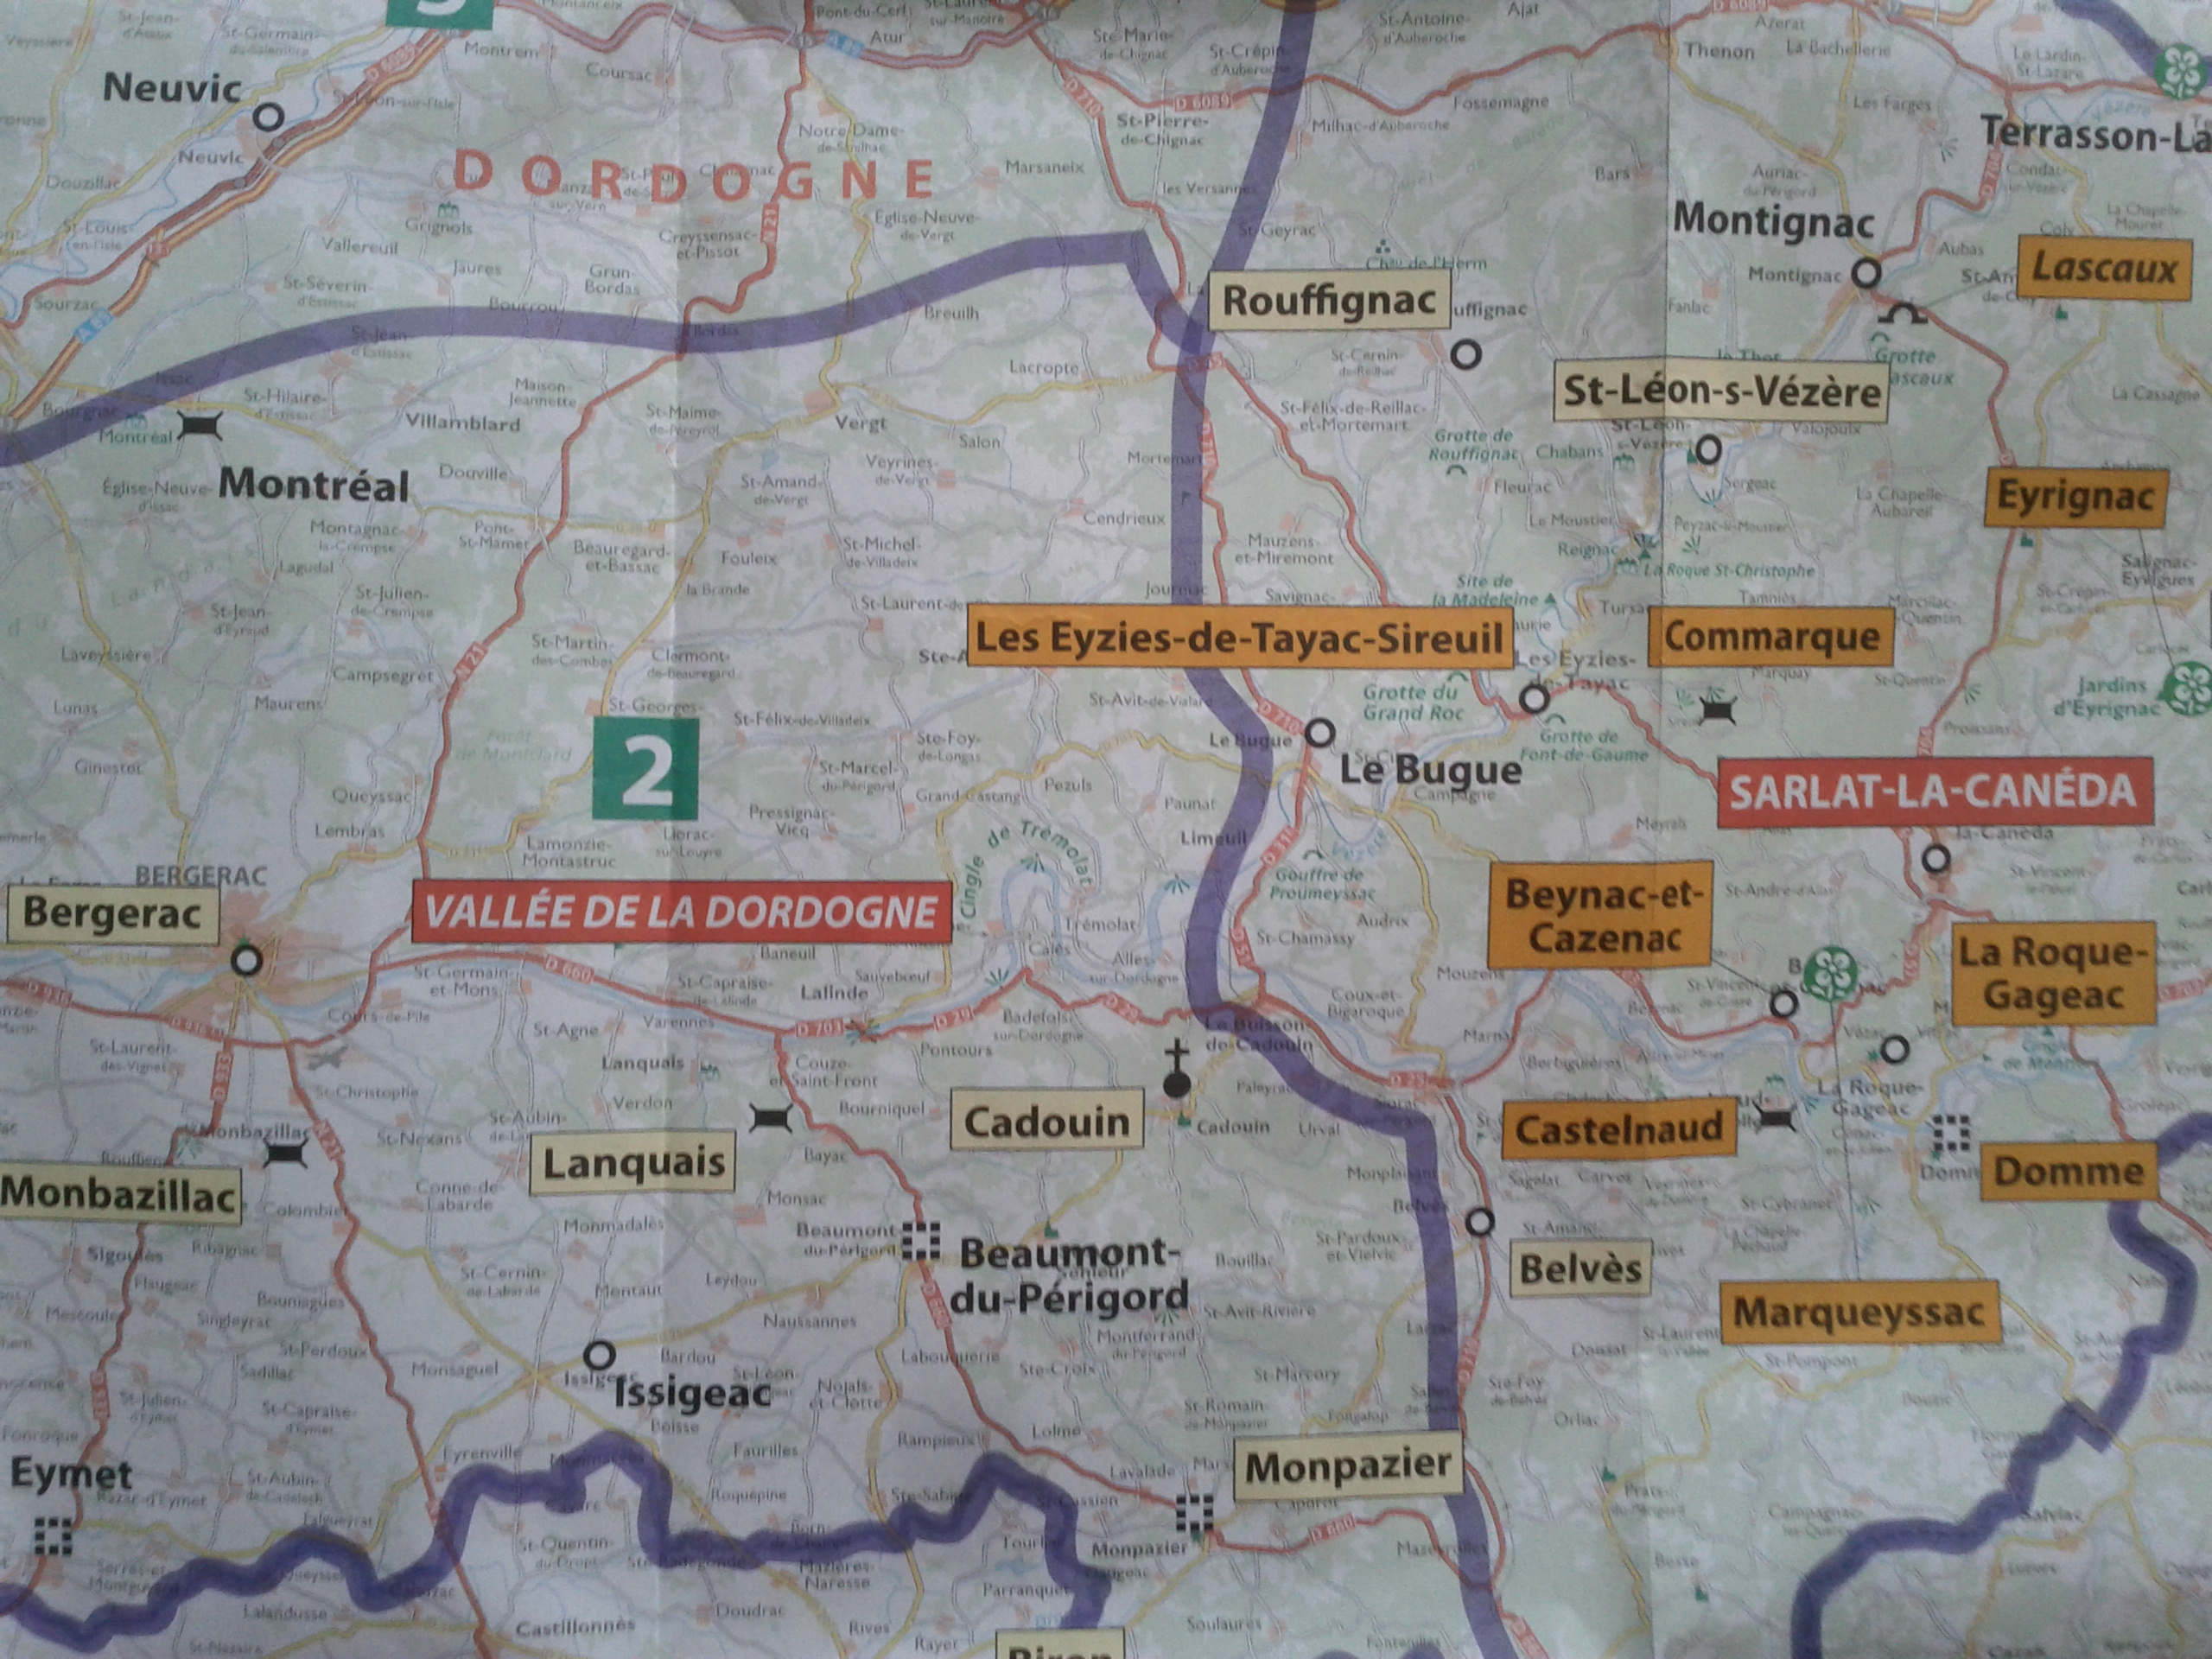
\includegraphics[scale=0.25]{carte_dordogne.ps}};
        \draw[very thin] (0,0) grid[xstep=0.5,ystep=0.5] (12,6.2);
        \coordinate (O) at (0,0); \draw (O) node[below left = -2pt] {$O$};
        \coordinate (I) at (0.5,0); \draw (I) node[below=1pt] {$I$} node {|};
        \coordinate (J) at (0,0.5); \draw (J) node[left] {$J$} node[below=-4pt] {--};
        \draw[thick,->] (-0.2,0) -- (12.4,0); \draw[thick,->] (0,-0.2) -- (0,6.4);
        \draw (5.5,1.5) node[scale=1.25] {$\bullet$} node[below left] {\textbf B};
        \draw (7.5,1.5) node[scale=1.25] {$\bullet$} node[above right] {\textbf P};
        \draw (7.5,1) node[scale=1.25] {$\bullet$} node[above right=-2pt] {\textbf R};
    \draw (8,4) node[scale=1.25] {$\bullet$} node[above left] {\textbf S};
    \end{tikzpicture}
\end{center}\medskip

L'unité de longueur est le carreau. Les distances entre deux villes sont calculées en ligne droite.

\begin{enumerate}
    \item Donner les coordonnées des points $O$ ; $I$ ; $J$ ; $R$ ; $B$ ; $S$ et $P$.
    \item Déterminer la longueur $BP$.
    \item À quelle distance, en ligne droite, la maison de Paul se situe-t-elle de La Roque-Gageac ?
    \item Expliquer pourquoi $BR = \sqrt{BP^2 + RP^2}$.
    \item Calculer alors la distance entre Beynac et La Roque-Gageac.
    \item Un oiseau part de la maison de Paul pour se rendre, en ligne droite, à Sarlat. Quelle est la distance parcourue ?
    \item Sachant que la distance réelle entre Sarlat et Beynac est d'environ $7{,}3~km$, en déduire alors la distance réelle que l'oiseau a parcourue.
\end{enumerate}

\end{document}
